\titleformat{\chapter}[display]
  {\normalfont\Large\bfseries}{\centering Tuần 9}{10pt}{\centering\Huge\bfseries}
  
\chapter{Nhập Môn Cơ Học Giải Tích}

Thống nhất các định luật để đưa về một quy luật chung cơ bản nhất là khát vọng của các nhà vật lý. Các lý thuyết về nguyên lý tác dụng tối thiểu, cơ học Lagrange và cơ học Hamilton được xem là những lý thuyết tiềm năng, cho phép mô tả các định luật về cơ học, thuyết tương đối, trường điện từ, cơ học lượng tử, v.v.

Trong giới hạn của cơ học cổ điển, các lý thuyết này có thể được xem là tương đương với cơ học Newton. Tuy nhiên, chúng có những ưu điểm riêng biệt, đặc biệt là trong việc giải quyết các bài toán liên quan đến chuyển động của hệ nhiều vật thể với hệ thống lực liên kết phức tạp.

\section{Nguyên lý tác dụng tối thiểu}

Theo nguyên lý tác dụng tối thiểu, các hệ vật lý luôn tuân theo một quy luật có hàm tác dụng \(S\) là cực tiểu.

Trên thực tế, ta có thể hiểu nguyên lý này là một hướng phát triển lý thuyết. Nói theo cách khác, nguyên lý này không phải là một định luật vật lý, mà là một phương pháp để xây dựng các định luật vật lý. Trong trường hợp một định luật vật lý mới khiến cho nguyên lý này không còn phù hợp, các nhà vật lý sẽ xem xét và hiệu chỉnh lại hàm tác dụng \(S\) để nó phù hợp với định luật mới.

Sự tiện lợi của nguyên lý biến phân và phương trình Euler-Lagrange là một động lực lớn để nguyên lý tác dụng tối thiểu tiếp tục được duy trì và phát triển trong quá trình xây dựng các lý thuyết vật lý mới.

\subsection{Nguyên lý biến phân}



\subsection{Phương trình Euler}

Xét một phiếm hàm \(S\) phụ thuộc vào một hàm số \(\mathbf{q}(t)\) và đạo hàm theo biến \(t\) của nó \(\mathbf{\dot{q}}\) với điều kiện biên xác định tại \(t_1\) và \(t_2\) theo biểu thức
\begin{equation}
    S \left[\mathbf{q}(t), \mathbf{\dot{q}}(t)\right] = \int_{t_1}^{t_2} L\left[ \mathbf{q}(t), \mathbf{\dot{q}}(t), t \right] \mathrm{d}t,
\end{equation}
trong đó \(L\left[ \mathbf{q}(t), \mathbf{\dot{q}}(t), t \right]\) là một hàm phụ thuộc vào hàm số \(\mathbf{q}(t)\), đạo hàm của nó \(\mathbf{\dot{q}}(t)\) và biến thời gian \(t\), được gọi là hàm Lagrange.

Với điều kiện biên xác định tại \(t_1\) và \(t_2\), việc hàm tác dụng \(S\) đạt cực tiểu phụ thuộc vào dạng hàm \(\mathbf{q}(t)\). Lấy biến phân của hàm tác dụng \(S\), ta có

\begin{equation} \label{eq:deltaS}
    \delta S = \int_{t_1}^{t_2} \left( \frac{\partial L}{\partial \mathbf{q}} \delta \mathbf{q} + \frac{\partial L}{\partial \mathbf{\dot{q}}} \delta \mathbf{\dot{q}} \right) \mathrm{d}t.
\end{equation}

Áp dụng định lý Leibniz cho biến phân \(\delta \mathbf{\dot{q}} = \mathrm{d}\left( \delta \mathbf{q} \right)\mathrm{d}t\)
\begin{equation}
    \dfrac{\partial L}{\partial \mathbf{\dot{q}}} \delta \mathbf{\dot{q}} = \frac{\partial L}{\partial \mathbf{\dot{q}}} \frac{\mathrm{d}}{\mathrm{d}t} \delta \mathbf{q} = \frac{\mathrm{d}}{\mathrm{d}t} \left( \frac{\partial L}{\partial \mathbf{\dot{q}}} \delta \mathbf{q} \right) - \frac{\mathrm{d}}{\mathrm{d}t} \left( \frac{\partial L}{\partial \mathbf{\dot{q}}} \right) \delta \mathbf{q}.
\end{equation}

Thế vào phương trình \eqref{eq:deltaS}, ta có

\begin{equation}
    \delta S = \int_{t_1}^{t_2} \left( \frac{\partial L}{\partial \mathbf{q}} - \frac{\mathrm{d}}{\mathrm{d}t} \left( \frac{\partial L}{\partial \mathbf{\dot{q}}} \right) \right) \delta \mathbf{q} \mathrm{d}t + \left[ \frac{\partial L}{\partial \mathbf{\dot{q}}} \delta \mathbf{q} \right] \Big|_{t_1}^{t_2}.
\end{equation}

Vì \(\delta S = 0\) với mọi hàm \(\delta \mathbf{q}\) đạt điều kiện biên xác định tại \(t_1\) và \(t_2\), nên ta có
\begin{equation} \label{eq:EL}
    \frac{\partial L}{\partial \mathbf{q}} - \frac{\mathrm{d}}{\mathrm{d}t} \left( \frac{\partial L}{\partial \mathbf{\dot{q}}} \right) = 0.
\end{equation}

Phương trình \eqref{eq:EL} được gọi là phương trình Euler, hay phương trình Euler-Lagrange, Lagrange loại 2 (đối với cơ học). 

Như vậy, phiếm hàm \(S\) đạt cực tiểu khi và chỉ khi hàm số \(\mathbf{q}(t)\) thỏa mãn phương trình Euler-Lagrange \eqref{eq:EL}.

\subsection{Phương trình tích phân Euler}

Xét hàm Lagrange \(L\) phụ thuộc vào một hàm số \(\mathbf{q}(t)\), đạo hàm theo biến \(t\) của nó \(\mathbf{\dot{q}}(t)\) và biến \(t\), đạo hàm toàn phần của hàm Lagrange theo biến \(t\) là
\begin{equation}
    \dfrac{\mathrm{d} L}{\mathrm{d} t} = \frac{\partial L}{\partial t} + \frac{\partial L}{\partial \mathbf{q}} \frac{\mathrm{d} \mathbf{q}}{\mathrm{d} t} + \frac{\partial L}{\partial \mathbf{\dot{q}}} \frac{\mathrm{d} \mathbf{\dot{q}}}{\mathrm{d} t}.
\end{equation}
Mặt khác
\begin{equation}
    \dfrac{\mathrm{d} }{\mathrm{d} t} \left( \mathbf{\dot{q}} \dfrac{\partial L}{\partial \mathbf{\dot{q}}} \right) = \dfrac{\mathrm{d} \mathbf{\dot{q}}}{\mathrm{d} t} \dfrac{\partial L}{\partial \mathbf{\dot{q}}} + \mathbf{\dot{q}} \dfrac{\mathrm{d}}{\mathrm{d} t} \left( \dfrac{\partial L}{\partial \mathbf{\dot{q}}} \right).
\end{equation}
Kết hợp hai biểu thức trên, ta có
\begin{equation}
    \dfrac{\mathrm{d} }{\mathrm{d} t} \left( \mathbf{\dot{q}} \dfrac{\partial L}{\partial \mathbf{\dot{q}}} \right) = \dfrac{\mathrm{d} L}{\mathrm{d} t} - \dfrac{\partial L}{\partial t} - \mathbf{\dot{q}} \left[ \dfrac{\partial L}{\partial \mathbf{q}} - \dfrac{\mathrm{d}}{\mathrm{d}t} \left( \dfrac{\partial L}{\partial \mathbf{\dot{q}}}\right) \right].
\end{equation}
Từ phương trình Euler-Lagrange \eqref{eq:EL}, thu gọn biểu thức trên, ta có
\begin{equation}
    \dfrac{\mathrm{d} }{\mathrm{d} t} \left( \mathbf{\dot{q}} \dfrac{\partial L}{\partial \mathbf{\dot{q}}} \right) = \dfrac{\mathrm{d} L}{\mathrm{d} t} - \dfrac{\partial L}{\partial t}.
\end{equation}
hay
\begin{equation}
    \dfrac{\partial L}{\partial t} - \dfrac{\mathrm{d} }{\mathrm{d} t} \left( L - \mathbf{\dot{q}} \dfrac{\partial L}{\partial \mathbf{\dot{q}}} \right) = 0.
\end{equation}

Trong trường hợp hàm Lagrange không phụ thuộc vào biến thời gian \(t\), tức là \(\partial L/\partial t = 0\), ta tìm được một đại lượng bảo toàn
\begin{equation}
    H = L - \mathbf{\dot{q}} \dfrac{\partial L}{\partial \mathbf{\dot{q}}}.
\end{equation}
Đại lượng này được gọi là tích phân Euler, hay trong cơ học giải tích là hàm Hamilton của hệ.

\subsection{Ứng dụng phương trình Euler: Nguyên lý Fermat trong quang học}

Nguyên lý Fermat trong quang học phát biểu rằng ánh sáng sẽ đi theo đường đi có thời gian truyền ánh sáng ngắn nhất giữa hai điểm. Để mô tả nguyên lý này bằng phương trình Euler, ta cần xác định hàm Lagrange cho hệ thống.

Giả sử ánh sáng truyền trong môi trường có chiết suất \(n\), thì thời gian truyền ánh sáng từ điểm \(A\) đến điểm \(B\) được tính bằng
\begin{equation}
    t = \int_{A}^{B} \frac{1}{c n}\mathrm{d}s,
\end{equation}
trong đó \(c\) là tốc độ ánh sáng trong chân không và \(\mathrm{d}s\) là độ dài vi phân của đường đi ánh sáng.

\textbf{Ví dụ 9.1: Định luật Snell.} Xét một tia sáng truyền qua một mặt phẳng từ điểm \(A\) đến điểm \(B\) với góc tới \(\theta_1\) và góc khúc xạ \(\theta_2\). Chiết suất của môi trường trước mặt phẳng là \(n_1\) và sau mặt phẳng là \(n_2\). 

\begin{figure}[!h]
    \centering
    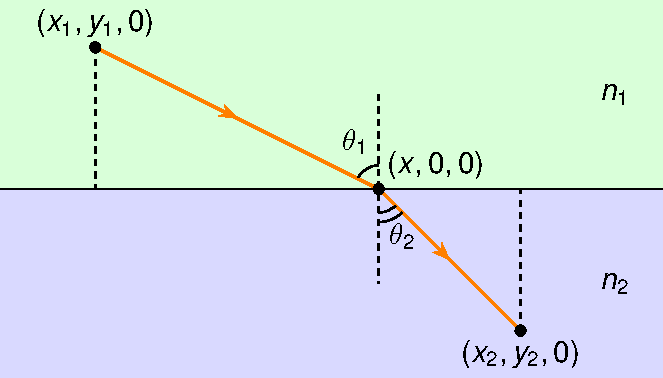
\includegraphics[width=0.7\textwidth]{Tuan9/Figures/Snellius_law.pdf}
    \caption{Tia sáng truyền qua hai môi trường có chiết suất khác nhau.}
    \label{fig:Snell_law}
\end{figure}
Chứng minh rằng tia sáng đi theo đường đi có thời gian truyền ánh sáng ngắn nhất giữa hai điểm \(A\) và \(B\) theo định luật Snell:
\begin{equation}
    n_1 \sin \theta_1 = n_2 \sin \theta_2.
\end{equation}

\textbf{Giải:} 

Thời gian truyền ánh sáng từ điểm \(A\) đến điểm \(B\) được tính bằng
\begin{equation}
    t = \dfrac{1}{c} \int_{A}^{B} n(x,y,z) \sqrt{1 + \left( \dfrac{\mathrm{d} x}{\mathrm{d} y}\right)^2 + \left( \dfrac{\mathrm{d} z}{\mathrm{d} y}\right)^2} \mathrm{d}y.
\end{equation}
Hay cụ thể trong bài toán này
\begin{equation}
    t = \dfrac{1}{c} \left[ \int_{y_1}^{0} n_1 \sqrt{1 + \left( \dfrac{\mathrm{d} x}{\mathrm{d} y}\right)^2 + \left( \dfrac{\mathrm{d} z}{\mathrm{d} y}\right)^2} \mathrm{d}y + \int_{0}^{-y_2} n_2 \sqrt{1 + \left( \dfrac{\mathrm{d} x}{\mathrm{d} y}\right)^2 + \left( \dfrac{\mathrm{d} z}{\mathrm{d} y}\right)^2} \mathrm{d}y \right] .
\end{equation}
Do biểu thức này không phụ thuộc tường minh vào \(x\) và \(z\) mà chỉ phụ thuộc vào đạo hàm bậc nhất của chúng theo \(y\) là \(x'\) và \(z'\), áp dụng phương trình Euler, ta có
\begin{equation}
    0 + \dfrac{\mathrm{d}}{\mathrm{d}y} \left[ n_1 \dfrac{x'}{\sqrt{1+x'^2+z'^2}}  + n_2 \dfrac{x'}{\sqrt{1+x'^2+z'^2}} \right] = 0.
\end{equation}
Dựa vào các công thức hình học lượng giác, ta biết rằng \(\sin \left( \theta_1 \right) = \dfrac{x'}{\sqrt{1+x'^2+z'^2}} \) với tại môi trường \(n_1\) và \(\sin \left( \theta_2 \right) = \dfrac{z'}{\sqrt{1+x'^2+z'^2}} \) tại môi trường \(n_2\). Do đó, ta có
\begin{equation}
    \dfrac{\mathrm{d}}{\mathrm{d}y} \left[ n_1 \sin \theta_1 = n_2 \sin \theta_2 \right] = 0 \Rightarrow n_1 \sin \theta_1 = n_2 \sin \theta_2 = \text{const}.
\end{equation}
Ta nhớ rằng, tại \(n_1 = n_2\) thì tia sáng truyền thẳng, tức là \(\theta_1 = \theta_2\), nên hằng số ở vế phải của biểu thức phải bằng 0. Do đó, ta có
\begin{equation}    
    n_1 \sin \theta_1 = n_2 \sin \theta_2.
\end{equation}

Đây chính là biểu thức của định luật khúc xạ Snell, mô tả sự khúc xạ của tia sáng khi truyền qua hai môi trường có chiết suất khác nhau.

Tổng quát hơn, với một môi trường có chiết suất \(n_y\) biến đổi liên tục theo tọa độ \(y\), ta có thể viết lại hàm Lagrange cho thời gian truyền ánh sáng như sau
\begin{equation}
    L = n(y) \sqrt{1 + \left( \dfrac{\mathrm{d} x}{\mathrm{d} y}\right)^2 + \left( \dfrac{\mathrm{d} z}{\mathrm{d} y}\right)^2}.
\end{equation}

Áp dụng phương trình Euler-Lagrange, ta có
\begin{equation}
    \frac{\partial L}{\partial x} - \frac{\mathrm{d}}{\mathrm{d}y} \left( \frac{\partial L}{\partial x'} \right)= 0.
\end{equation}
hay
\begin{equation}
    \dfrac{\mathrm{d}}{\mathrm{d} y} \left[ n(y) \dfrac{x'}{\sqrt{1+x'^2+z'^2}} \right]= 0 \Rightarrow n(y) \sin \theta = \text{const}.
\end{equation}

\textbf{Ví dụ 9.2: Chiết suất biến đổi cầu.} Một môi trường có chiết suất đối xứng cầu biến đổi theo bán kính \(n(r)\). Chứng minh rằng quỹ đạo của tia sáng tuân theo phương trình
\begin{equation}
    n(r) r \sin \left( i \right) = \text{const}.
\end{equation}
với \(i\) là góc tạo bởi tia tới và đường bán kính tại vị trí cách tâm \(r\).

\subsection{Ứng dụng phương trình Euler: Các hệ cân bằng tĩnh tại vị trí có thế năng cực tiểu}

Ta biết rằng, khi một hệ cơ học cân bằng tĩnh, thế năng của hệ đạt cực tiểu. Ở các cơ hệ chứa các phần tử phân bố theo tọa độ, ta thường quan sát thấy thế năng được viết dưới dạng một phiếm hàm tích phân phụ thuộc vào hàm phân bố của các phần tử trong hệ. Tức là
\begin{equation}
    U = \int L \mathrm{d}x,
\end{equation}
trong đó \(L\) là hàm Lagrange phụ thuộc vào hàm phân bố của các phần tử trong hệ và các đạo hàm của nó theo biến \(x\).

\textbf{Ví dụ 9.3: Catenary.} Xét một dây treo giữa hai điểm \(A\) và \(B\) với chiều dài dây là \(L\) và khoảng cách giữa hai điểm là \(d\). Chứng minh rằng hình dạng của dây treo là một đường cong catenary, tức là đường cong có phương trình
\begin{equation}
    y = a \cosh \left( \frac{x}{a} \right),
\end{equation}
trong đó \(a\) là một hằng số phụ thuộc vào chiều dài dây và khoảng cách giữa hai điểm.

\textbf{Ví dụ 9.4: Mặt bong bóng (TST 2012)} 

\section{Cơ học Lagrange}

\subsection{Nguyên lý D'Alembert về công ảo}



\subsection{Động lượng suy rộng}

\subsection{Giải phương trình chuyển động bằng phương pháp Runge-Kutta 4}

\subsection{Tính toán lực bị động dựa trên phương trình Lagrange loại 2}


\section{Định lý Noether}

% Continuous symmetry

% Bài tập ví dụ: Xác định phương trình vi phân mô tả chuyển động của con lắc kép.

\section{Các lý thuyết cơ học giải tích khác}

\subsection{Cơ học Hamilton}

\subsection{Nguyên lý Gauss về liên kết tối thiểu}

\subsection{Phương trình Appell cho cơ hệ phi Holonom}


\section{Bài tập}

\textbf{Bài 9.1:} Xét một hàm tác dụng \(S\) phụ thuộc vào một hàm số \(\mathbf{q}(t)\) và các đạo hàm theo biến \(t\) của nó \(\mathbf{\dot{q}}(t)\), \(\mathbf{\ddot{q}}(t)\), \ldots, \(\mathbf{q}^{(n)} (t)\) với điều kiện biên xác định tại \(t_1\) và \(t_2\) theo biểu thức
\begin{equation}
    S \left[\mathbf{q}(t), \mathbf{\dot{q}}(t), \ldots, \mathbf{q}^{(n)} (t)\right] = \int_{t_1}^{t_2} L\left[ \mathbf{q}(t), \mathbf{\dot{q}}(t), \ldots, \mathbf{q}^{(n)} (t), t \right] \mathrm{d}t,
\end{equation}
chứng minh rằng hàm tác dụng \(S\) đạt cực tiểu khi và chỉ khi hàm số \(\mathbf{q}(t)\) thỏa mãn phương trình Euler-Lagrange tổng quát
\begin{equation}
    \frac{\partial L}{\partial \mathbf{q}} - \frac{\mathrm{d}}{\mathrm{d}t} \left( \frac{\partial L}{\partial \mathbf{\dot{q}}} \right) + \dfrac{\mathrm{d}^2}{\mathrm{d} t^2} \left( \dfrac{\partial L}{\partial \mathbf{\ddot{q}}}\right) - \cdots + (-1)^n \frac{\mathrm{d}^n}{\mathrm{d}t^n} \left( \frac{\partial L}{\partial \mathbf{q}^{(n)}} \right) = 0.
\end{equation}

\textbf{Bài 9.2:} Xét một cơ hệ có hàm Lagrange \(L ( q, \ddot{q}, t)\) có dạng
\begin{equation}
    L = -\dfrac{1}{2} m q \ddot{q} - \dfrac{1}{2} k q^2,
\end{equation}
Xác định phương trình chuyển động của cơ hệ này bằng phương pháp Euler-Lagrange.

\textbf{Bài 9.3:} (Bài 2 Rudolf Ortvay Competition in Physics 2022) Giải phương trình quỹ đạo của một hệ có hàm Lagrange
\begin{equation}
    L (x, \dot{x}, y, \dot{y}, z, \dot{z}) = x^2 y^2 \dot{z}^2 + \dfrac{x^2 \dot{y}^2}{1-y^2} + \dot{x}^2.
\end{equation}
Liệu có hệ vật lý nào được mô tả bởi hàm Lagrange như trên không?

\section{Lời giải}


\begin{refsection}
\nocite{cline2017variational,morin2008introduction,kompaneyets2013theoretical,dao2002cohocgiaitich}
\printbibliography
\end{refsection}